\section{Parallel coordinate descent methods}\label{pcdm}
In this section, we introduce the parallel coordinate descent algorithm, which benefits significantly from our $PSF$ approximation scheme. The $PSF$ approximation we developed lets the deconvolution algorithm use an approximate $PSF$. It uses only the center window of the full $PSF$, where each side of the window is a fraction of the full $PSF$. Or in other words: The approximation method resulted in a sparse $PSF$ for the deconvolution algorithm. We use the introduced sparsity for parallel deconvolutions, resulting in the parallel coordinate descent algorithm

The serial coordinate descent algorithm minimizes a single pixel in each iteration. Parallel coordinate descent methods can minimize multiple pixels in parallel in each iteration. This section, we introduce the parallel coordinate descent deconvolution algorithm. We created two implementations: One implementation is more general, it uses gradient acceleration to speed up convergence, and can group multiple pixels into blocks. It is a parallel algorithm, which can minimize multiple blocks in parallel in each iteration. But grouping pixels into blocks and gradient acceleration did not lead to an overall faster deconvolution algorithm. This section focuses on our second implementation, which is not accelerated and can only optimize pixels instead. The introduction of the accelerated, parallel, block coordinate descent algorithm and its results can be found in the attachments.

The parallel coordinate descent algorithm can update multiple pixels in parallel. However, if it updates pixels which are next to each other in the image, their $PSF$s overlap and it over-estimates their pixel values. This can lead the parallel algorithm to diverge. In section \ref{pcdm:pcdm:eso} we introduce the core concept of parallel coordinate descent methods: The Estimated Separability Overapproximation (ESO). We then show how the parallel coordinate descent algorithm can be implemented in an asynchronous manner in Section \ref{pcdm:async}. Parallel coordinate descent algorithms have been developed with a random selection strategy in mind. However, a random selection strategy does not perform well on the deconvolution problem. We demonstrate the problem of random selection and introduce our own solution in Section \ref{pcdm:adaption}.


\subsubsection{Estimated Separability Overapproximation (ESO)} \label{pcdm:pcdm:eso}
So far, we introduced a serial coordinate descent algorithm. If we want to update pixels in parallel, we need to estimate how much the $PSF$s of parallel updates 'overlap'. For example: If we update two pixels in parallel, and their combined $PSF$s do not overlap, then the update is independent. Updating the first pixel, and then the second pixel in a serial algorithm leads to the same result as updating both pixels in parallel. 

However, if we update two pixels, which are located next to each other in the image, then their combined $PSF$s overlap significantly. Their updates are dependent on each other. If we update the first pixel, and then the second pixel in a serial algorithm results in significantly lower pixel values for the second pixel. Because their $PSF$s overlap, both pixels try to explain mostly the same emission. If we update both pixels in parallel, each pixel would try to explain the same emission, and we would over-estimate their pixel values.

This over-estimation can lead to a diverging algorithm. To guarantee the convergence of a parallel pixel coordinate descent, we need to estimate the overlap of the $PSF$s of parallel updates. This can be done with the Estimated Separability Overapproximation (ESO) developed in \cite{richtarik2016parallel}. The ESO estimates how much the $PSF$s overlap, if we update $\tau$ random pixels in parallel:

\begin{equation}\label{pcdm:pcdm:eso}
ESO(\omega, \tau, n) = 1+ \frac{(\omega - 1)(\tau - 1)}{max(1, n -1)}
\end{equation}

Where $\omega$ is the number of non-zero entries in the $PSF$, $\tau$ is the number of random parallel updates in each iteration, and $n$ is the number of pixels in the image. Let us use an example to demonstrate what the ESO means: Let us assume the $PSF$ has $\omega = 24$ non zero entries, $\tau = 4$ processors to update in parallel, and the image is $64^2$ pixels in size. Plugging the values into the ESO gives us the following result:

\begin{equation}
ESO(\omega = 24, \tau = 4, n = (64^2) = 1+ \frac{(24 - 1)(4 - 1)}{max(1, 4096 -1)} \approx 1.017
\end{equation}

An ESO of $1$ means the $\tau = 4$ parallel updates are completely independent of each other, and we do not need to account for overlapping $PSF$s. In our example, we arrived at an ESO of $1.017$. This means every parallel update step has to be divided by $1.017$ to account for overlapping $PSF$s, and ensure convergence.

The ESO only needs to know the number of non-zero components. It is independent of the exact structure of the $PSF$. The fewer non-zero components the $PSF$ has, the closer it is to 1, and the more effective each parallel update is. The ESO benefits from our $PSF$ approximation. It decreases the number of non-zero components in the $PSF$ and leads to an ESO closer to 1.

However, note that the ESO assumes we choose $\tau = 4$ pixels uniformly at random. Indeed, a uniform random selection strategy is a core assumption for the parallel coordinate descent method\cite{richtarik2016parallel}. Random selection strategies tend to perform badly on the deconvolution problem. Later in Section \ref{pcdm:adaption}, we develop a pseudo-random selection strategy which does not break the random selection assumption of the ESO, but performs better on the deconvolution problem.


\subsection{Asynchronous parallel coordinate descent algorithm.}\label{pcdm:async}
So far, we introduced the serial coordinate descent and the ESO. The serial block coordinate descent can update a pixel in a single iteration, and the ESO estimates how much $PSF$s overlap when we perform parallel update steps. In this section, we put the ESO and the serial algorithm together into a parallel coordinate descent algorithm based on APPROX\cite{fercoq2015accelerated}. The implementation is asynchronous, meaning each processor chooses its pixel to minimize, and updates the gradient map independently of the other processors.

In this project, we use a $\tau$-nice uniform sampling, which can be easily implemented with asynchronous processors: Each of the $\tau$ processors chooses its pixel to minimize uniformly at random. The asynchronous processors are only forbidden to select the same pixel. To ensure this in the parallel algorithm, we introduce a new array: The 'pixelLocks'. Each asynchronous processor writes its processor ID in the pixelLocks map for the pixel it is currently updating. If there is already a processor ID written at the specific location, the processor simply selects another random pixel. 

The write to the pixelLocks array can be easily implemented with a compare-exchange operation. Compare-exchange is an atomic instruction on modern computing hardware.  It checks for a value at a specific memory location. If the check returns true, it exchanges the value at the memory location. The compare-exchange instruction is atomic, meaning there cannot be another process which has modified the memory location in the meantime. This leads us to the following algorithm:

\begin{lstlisting}
dirty = IFFT(GridVisibilities(visibilities))
residualsPadded = ZeroPadding(dirty)

psfPadded = ZeroPadding(PSF)
psfPadded = FlipUD(FlipLR(psfPadded))
gradientUpdate = iFFT(FFT(ZeroPadding(PSF)) * FFT(psfPadded))

x = new Array[,]
gradientsMap = iFFT(FFT(residualsPadded) * FFT(psfPadded))
lipschitzMap = CalcLipschitz(PSF)

eso = ESO(CountNonZero(PSF), t, x.Length)

concurrentIterations = 1000 / t
pixelLocks = new Array[,]

do 
	//asynchronous iterations
	parallelDiffs = new Array[]
	parallel for each processorId in (0:t)+1
		for concurrentIter in 0:concurrentIterations
			pixelLocation = AtomicLockRandomPixel(pixelLocks, processorId)
			
			//Step 2: update pixel asynchronously
			lipschitz = LipschitzMap[pixelLocation]
			lipschitz = lipschitz * eso
			
			oldValue = x[pixelLocation]
			tmp = gradientsMap[pixelLocation] + oldValue * lipschitz
			optimalValue = Max(tmp - lambda*alpha) / (lipschitz + (1 - alpha)*lambda)
			diff = optimalValue - oldValue
			
			parallelDiffs[processorId -1] = Max(parallelDiffs[processorId -1], diff)
			
			//Step 3: Update gradients asynchronously
			shiftedUpdate = Shift(gradientUpdate, pixelLocation)
			AtomicSum(gradientsMap, -shiftedUpdate * diff)
	
			//unlock pixel
			pixelLocks[pixelLocation] = 0
	maxParallelDiff = Max(parallelDiffs)
while maxParallelDiff  < epsilon

\end{lstlisting}

Each of the $\tau$ processors performs a number of iterations independently of the other processors. This is what we call an asynchronous 'batch' of iterations. In each asynchronous iteration, a single processor chooses a pixel to minimize uniformly at random, which is not locked by a different processor. We multiply the Lipschitz constant with the ESO, which ensures convergence for parallel updates. The gradient map gets updated asynchronously. Each processor writes its changes atomically to memory. We also implemented the atomic sum with a compare-exchange operation on the CPU.

%On modern CPU's, we can use the compare-exchange instruction to ensure atomic writes/updates on the pixelLocks and the two gradient maps. If a processor selects a pixel which does not overlap with the $PSF$ of another selected pixel, it can update the pixel with minimal communication costs. In our deconvolution problem, the chance that two processors update the same position in the gradient maps at the same time depends on the size of the $PSF$. The smaller the $PSF$, the smaller the chance is that more than one processor tries to update the same position.

With an asynchronous implementation, our parallel coordinate descent algorithm benefits in two ways from a smaller $PSF$: First, a smaller $PSF$ leads to an ESO closer to 1. With an ESO close to 1, our parallel updates become as efficient as the equivalent number of serial updates. And second, by decreasing the chance of two processors updating the same memory location at the same time, it decreases the communication cost of the algorithm.


\subsection{The problem with random selection for deconvolution} \label{pcdm:adaption}
Our parallel coordinate descent algorithm developed in this section does not perform well on the deconvolution problem. The reason lies in the random selection strategy: In the first few iterations, the deconvolution algorithm selects pixels at random, and tries to explain the whole emission in that area. The emission in this area of the image is 'locked' inside a few pixels. Before the parallel algorithm can make a meaningful update to a neighboring pixel, it first needs to select the same pixel again. In short, the first iterations always over-estimate the pixel values, which leads to slow convergence rates. 

\begin{figure}[h]
		\centering
	\begin{subfigure}[b]{0.245\linewidth}
		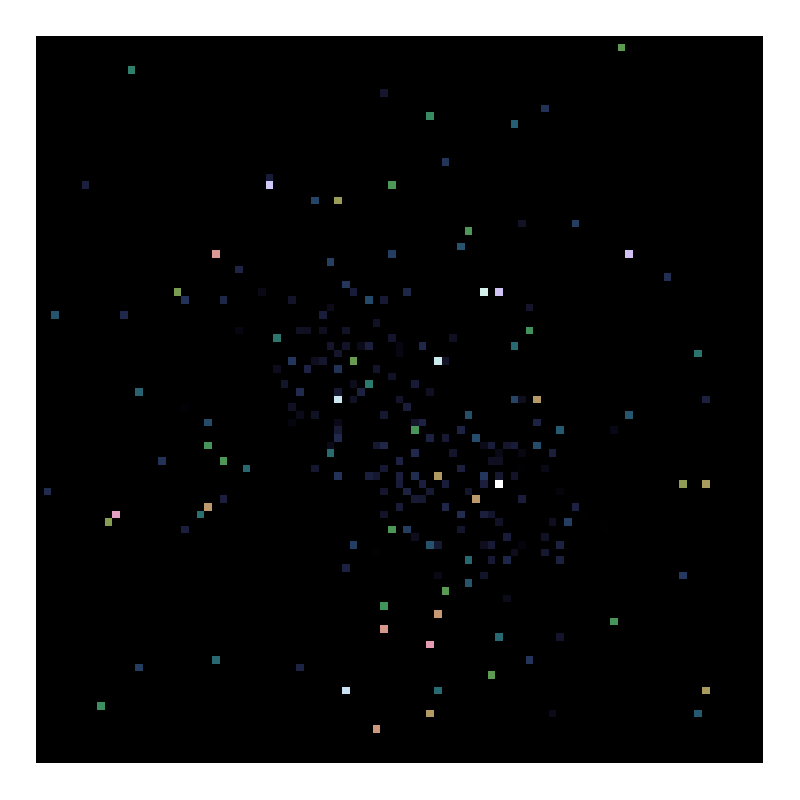
\includegraphics[width=1.00\linewidth, clip, trim= 0.25in 0.25in 0.25in 0.25in]{./chapters/05.pcdm/randomProblem/random_1k_block1.png}
		\caption{8k iterations}
		\label{pcdm:adaption:randomProblem:block11}
	\end{subfigure}
	\begin{subfigure}[b]{0.245\linewidth}
		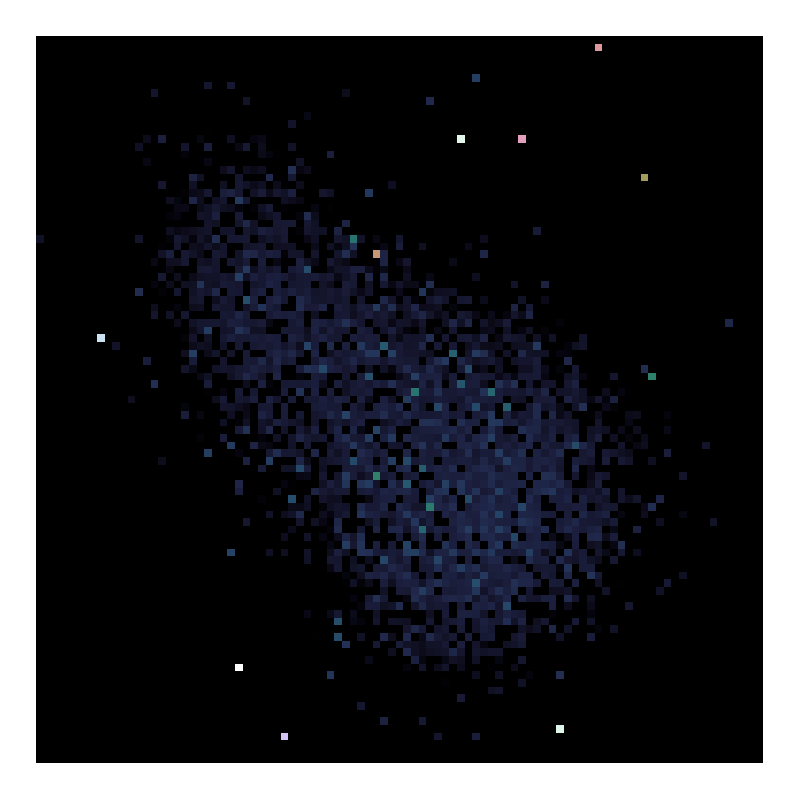
\includegraphics[width=1.00\linewidth, clip, trim= 0.25in 0.25in 0.25in 0.25in]{./chapters/05.pcdm/randomProblem/random_10k_block1.png}
		\caption{80k iterations}
		\label{pcdm:adaption:randomProblem:block12}
	\end{subfigure}
		\begin{subfigure}[b]{0.245\linewidth}
		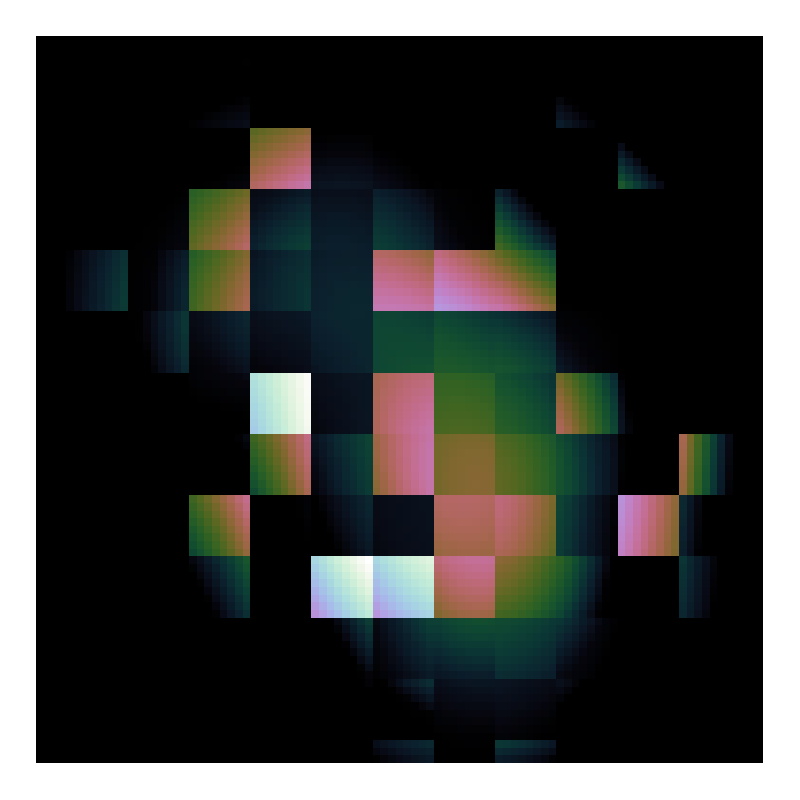
\includegraphics[width=1.00\linewidth, clip, trim= 0.25in 0.25in 0.25in 0.25in]{./chapters/05.pcdm/randomProblem/random_1k_block8.png}
		\caption{8k iterations, $8^2$ block}
		\label{pcdm:adaption:randomProblem:block81}
	\end{subfigure}
		\begin{subfigure}[b]{0.2405\linewidth}
		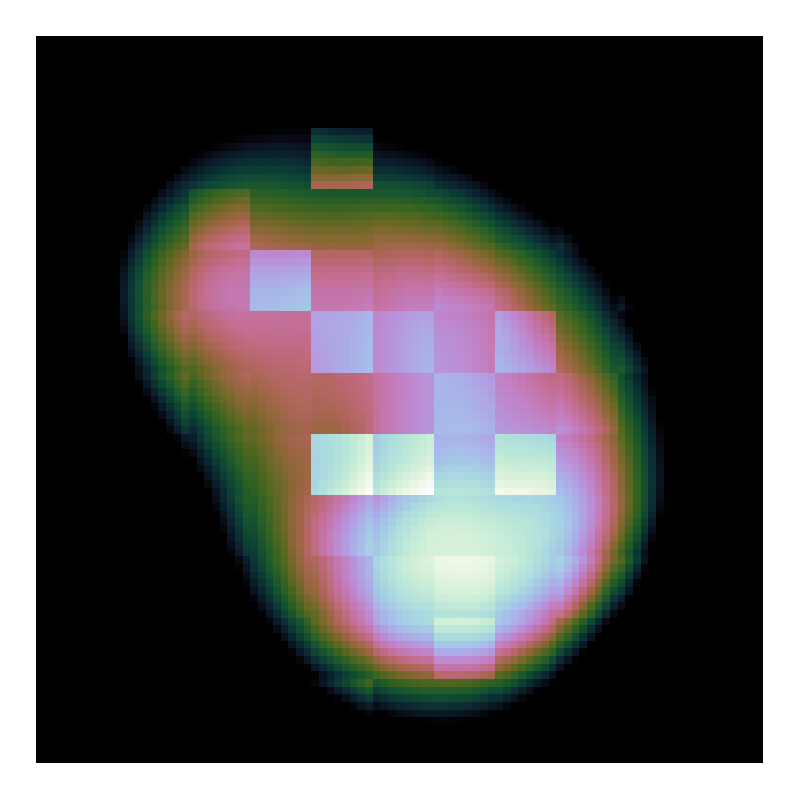
\includegraphics[width=1.00\linewidth, clip, trim= 0.25in 0.25in 0.25in 0.25in]{./chapters/05.pcdm/randomProblem/random_10k_block8.png}
		\caption{80k iterations, $8^2$ block}
		\label{pcdm:adaption:randomProblem:block82}
	\end{subfigure}
	\caption{Random parallel deconvolutions on the LMC N132D supernova remnant.}
	\label{pcdm:adaption:randomProblem}
\end{figure}

The Figure \ref{pcdm:adaption:randomProblem} shows the behavior on the LMC observation. The reconstructions receive obvious artifacts from the random selection strategy. The pixels, which get selected in the first few iterations, keep their over-estimated values. The parallel algorithm needs to select them several times to reduce their value. That is why even after 80k iterations, the N132D supernova remnant gets only hinted at in Figure \ref{pcdm:adaption:randomProblem:block12}. Until the over-estimated pixels get selected again, the algorithm cannot do useful updates in that region.

This behavior is pronounced when we choose a block size of one pixel (i.e. we do not group pixels into blocks). A naive solution is to increase the block size. This leads to fewer possible blocks in the image, and obviously an increased chance to select the same block again in later iterations. But as we see in Figure \ref{pcdm:adaption:randomProblem:block82}, the same problem exists with larger block sizes, although less pronounced. After 80k iterations the N132D supernova remnant is visible, but a few random blocks still contain too much of the emission in that area.

A random selection strategy needs a prohibitive large number of iterations to converge. But we cannot simply switch out the selection strategy. The random selection strategy is at the core of the Parallel coordinate descent methods. Remember the ESO arises from the fact that we select $tau$ pixels uniformly at random. When we select $\tau$-pixels with a greedy strategy, we might break the ESO, and the parallel algorithm may not converge at all.

To solve this behavior, we introduce the pseudo-random selection strategy:  We select a pixel at random, but greedily search in the neighborhood for the optimal pixel to optimize. The size of the neighborhood can be defined by the user as the 'Search Factor' parameter. It is essentially a mix between a greedy and a random selection strategy. If we choose a Search Factor of $1.0$, the neighborhood is the whole image, and we arrive at a greedy strategy. If we choose a Search Factor of $0.0$, then the neighborhood is one pixel, and we are back at a random strategy. The mixture of the greedy and random strategy allows us to fix the problems with the pure random strategy, without breaking any assumptions from the ESO. The optimal value for the Search Fraction is explored later in Section \ref{pcdm:results:fraction}.

We have developed three related extensions, which speed up the parallel coordinate descent algorithm in practice. We use an active set, a restarting strategy, and a 'Minor' cycle. The active set only allows the parallel algorithm to choose from a subset of pixels, which are likely to be non-zero in the final image. The restarting strategy resets the active set when it may not contain relevant pixels. Restarting is an important strategy for gradient accelerated algorithms, which have not been discussed in this section. Lastly, we re-introduce a 'Minor' cycle. The parallel coordinate descent algorithm can exploit our $PSF$ approximation scheme. With increasingly small $PSF$ windows, the parallel algorithm achieves ever faster convergence times. But the downside is it also requires more Major cycles to converge. To combat this problem, we periodically reset the residual image: We convolve the intermediate solution with the full $PSF$, and subtract it from the residuals. This is what we call a 'Minor' cycle. How these three extensions work in detail can be found in the attachments.




